\documentclass[11pt, oneside]{book}
\usepackage[pdftex,a4paper]{geometry}
\usepackage{pdfpages}
\usepackage{graphicx}
\usepackage{amssymb}

\pagestyle{empty}

\usepackage[scaled]{helvet}
\renewcommand\familydefault{\sfdefault} 
\usepackage[T1]{fontenc}


\usepackage{ifthen}
\usepackage{float}
\usepackage{calc}
\usepackage[export]{adjustbox}% http://ctan.org/pkg/adjustbox
\usepackage{xstring}
\usepackage{multicol}

% Extract a symbol from the ISO document. And show it together with the title and warning text.
%
% Params:		Page with the symbol on it.
%			Title
%			Warning text
%			Y height on the page.
%
\newcommand{\decal}[5]{
\begin{minipage}{\linewidth}
	\begin{minipage}[t]{0.3\textwidth}
	       \vspace{0pt}
	       % The ISO document has a 'gutter' - so we shift the X a bit on the left/right page.
	       %
		\ifthenelse{\isodd{#1}}{
			\includegraphics[width=0.9\textwidth,page=#1,viewport=103 #3 291 #4,clip=true]{13GR_PistopioimeniSimansi_ISO_7010.pdf}
		}{
			\includegraphics[width=0.9\textwidth,page=#1,viewport=70 #3 261 #4,clip=true]{13GR_PistopioimeniSimansi_ISO_7010.pdf}
		}
	\end{minipage}
	\begin{minipage}[t]{0.6\textwidth}
		\setlength{\parindent}{4em}
		\setlength{\parskip}{1.2em}
	       \vspace{0pt}\raggedright
		{\LARGE \textbf{#2}}
	
		#5
		\vspace{1cm}
	\end{minipage}
\end{minipage}
}

% Turns out that the symbols are a bit shifted in the Y position or size depending on what
% class they are. So we split them into the three sections that have height differences.
%
% Params:		Page with the symbol on it.
%			Title
%			Warning text
%
\newcommand{\action}[3]{\decal{#1}{#2}{520}{715}{#3}}
\newcommand{\prohib}[3]{\decal{#1}{#2}{495}{690}{#3}}
\newcommand{\warn}[3]{\decal{#1}{#2}{520}{715}{#3}}

% A full page with a machine on it.
%
% Params:		Machine name
%			Tokens for standard instrutions: Zero or more from
%				Approval		Trustee approval needed.
%				Noise		Not after 19:00
%				Two			Two people required
%				Log			use must be logged
%				Dewalt		Attach dewalt dutch extractor.
%			Specific instructions 
%			Warnings, Symbols
%			Extra footer/bottom of the page text
%
\newcommand{\machinePage}[5]{%
\begin{center}
	\vspace{0cm}
	{\fontsize{50}{60} \textbf{#1}}
 
	\action{49}{\textbf{%
 		\IfSubStr{#2}{Approval}%
			{Instructions \& Approval Mandatory}
			{Instructions Mandatory}%
		}}
		{%
			Instructions \textbf{prior} to use are mandatory. Check the wiki for whom can help you.
			
			#3

		\IfSubStr{#2}{Noise}{Machine can only be used between 07:00 - 19:00 (be kind to our neighbours).}{}

		\IfSubStr{#2}{Approval}{Must have the `dangerous equipment waiver' filed with the foundations trustees and been given approval or card access.}{}

		\IfSubStr{#2}{Two}{A second person must be present during operation. This person must have agreed to be your second and needs to know how to stop the machine.}{}

		\IfSubStr{#2}{Log}{Report any use in the log - and \textbf{pay for it}!}{}

		\IfSubStr{#2}{Dewalt}{Be sure to attach and power on the dust extractor.}{}
	}
	\begin{multicols}{2}#4\end{multicols}
	
	\vspace{0.2cm}
	#5

	If the machine is not clean or appears broken - then report this to the mailing list. Clean/fix prior to use.

	\textbf{Report any damage, issues or accident within 24 hours to the mailing list.}
\end{center}
\vfill
\tiny \today
\pagebreak
}



% Use as much of the page as we can.
\setlength{\parindent}{4em}
\setlength{\parskip}{1.2em}
\setlength{\textheight}{28cm}
\setlength{\textwidth}{19cm}
\setlength{\hoffset}{-2cm}
\setlength{\voffset}{-2cm}

\begin{document}

%%%%%%%%%%%%%%%%%%%%%%%%%%%%%%%%%%%%%%%%%%
\machinePage{Large CNC Cutter}{Noise}{
	Be very careful with viruses/media -- as we cannot re-install the software on the PC.
}{
\action{51}{Ear protection strongly recommended}{Note also that this machine should not be used after 19:00}
\action{52}{Eye protection recommended}{Especially when using very small cutters.}
\action{64}{Wear a mask when needed}{Especially when cutting materials such as MDF}
\warn{124}{Machine can suddenly start}{%
	Machine can suddenly start moving; and can move under its own command (even when the PC is off).
	
	It will also start moving without warning when the PC is started/the software is started}
\warn{125}{Crushing}{Risk of crushing - the machine does not have any sensors that detect obstacles
This includes things such as your hands (do not lean on the blue rail) or tools you've left on the workspace.
}
}{
This machine contains commercial software which is locked to this specific hardware and OS install. Neither of which we can re-install (as we have no media and the suppliers have long gone out of business). So be very very careful with USB sticks and other media. A virus or malware may permanently kill this setup.
}

%%%%%%%%%%%%%%%%%%%%%%%%%%%%%%%%%%%%%%%%%%
\machinePage{Abene Mill}{Approval}{
}{
\prohib{100}{Do not wear gloves}{Especially strong leather ones. They get caught easily and then `help' ripping body parts off.}
\action{52}{Eye protection recommended}{Swarf will fly. Cutters can come loose. Broken cutters can fly very far and are razor sharp.}
\action{58}{Wear protective clothing}{Wear tight fitting clothing, keep long hair out tied up, no jewellery or anything else that can be caught by the machine.}
\warn{125}{Crushing}{Risk of crushing - the machine does not have any sensors that detect obstacles.

Note that it can also run very slow; barely noticeable.}
\warn{117}{Slippery surface}{Floor will get very slippery; especially when using coolant.}
\warn{128}{Sharp rotating elements}{This machine is essentially a cutter without any guard whatsoever.}
}{
Only switch XYZ feeds when the machine is not running. Use the handwheel to get the gear fully locked in prior to starting the feed. Be sure to tighten all 4 nuts post rotating the head or all 4 nuts when moving the head laterally.

Try to avoid getting coolant or similar on the slide-ways - especially the Y slipway between machine and table. Use a shield or adjust the flow. Machine needs to be cleaned post use.  When using coolant - also empty the recess on the left of the table and clean out the t-Slots until dry.
}

%%%%%%%%%%%%%%%%%%%%%%%%%%%%%%%%%%%%%%%%%%
\machinePage{Metal Lathe}{Approval}{
Be careful when using the auto-feed; especially with cutters near the revolving head.
}{
\prohib{100}{Do not wear gloves}{Especially strong leather ones. They get caught easily and then `help' ripping body parts off.}
\action{52}{Eye protection recommended}{Swarf will fly. Cutters can come loose. Broken cutters can fly very far and are razor sharp.}
\action{58}{Wear protective clothing}{Wear tight fitting clothing, keep long hair out tied up, no jewellery or anything else that can be caught by the machine.}
\warn{125}{Crushing}{Risk of crushing - the machine does not have any sensors that detect obstacles.

Note that it can also run very slow; barely noticeable.}
\warn{117}{Slippery surface}{Floor may get slippery when using coolant.}
% \warn{128}{Sharp rotating elements}{This machine is essentially a cutter without any guard whatsoever.}
}{
Clean after use - especially when you have used coolant or have used metals that can rust easily or cause a galvanic reaction.
}
%%%%%%%%%%%%%%%%%%%%%%%%%%%%%%%%%%%%%%%%%%
\machinePage{Wood Lathe}{Approval}{
This machine is for WOOD only.
}{
\action{64}{Wear a mask when needed}{Especially when cutting materials such as MDF}
\action{58}{Wear protective clothing}{Wear tight fitting clothing, keep long hair out tied up, no jewellery or anything else that can be caught by the machine.}
\action{52}{Eye protection mandatory}{}
\prohib{100}{Not recommended to wear gloves}{}
}{
}

%%%%%%%%%%%%%%%%%%%%%%%%%%%%%%%%%%%%%%%%%%
\machinePage{Mitre saw}{Noise}{
This machine is for WOOD only.

}{
\action{58}{Wear protective clothing}{Wear tight fitting clothing, keep long hair out tied up, no jewellery or anything else that can be caught by the machine.}
\action{52}{Eye protection recommended}{}
\action{51}{Ear protection recommended}{Note also that this machine should not be used after 19:00 if it is that noisy}
\action{64}{Wear a mask when needed}{Especially when cutting materials such as MDF}
\warn{128}{Sharp rotating elements}{So keep your fingers awa. Bypassing or using your fingers to hold the guard open is downright stupid.}
}{}

%%%%%%%%%%%%%%%%%%%%%%%%%%%%%%%%%%%%%%%%%%
\machinePage{Wood Circlesaw Table}{Approval,Noise,Two,Dewalt}{
This machine is for WOOD only.
}{
\action{51}{Ear protection strongly recommended}{Note also that this machine should not be used after 19:00}
\action{58}{Wear protective clothing}{Wear tight fitting clothing, keep long hair out tied up, no jewellery or anything else that can be caught by the machine.}
\action{52}{Eye protection recommended}{Especially when using very small cutters.}
\action{64}{Wear a mask when needed}{Especially when cutting materials such as MDF}
\prohib{100}{Do not wear gloves}{Especially strong leather ones. They get caught easily and then `help' ripping body parts off.}
}{
}

%%%%%%%%%%%%%%%%%%%%%%%%%%%%%%%%%%%%%%%%%%
\machinePage{Wood Bandsaw}{Approval,Dewalt}{
This machine is for WOOD only.
}{
\action{51}{Ear protection strongly recommended}{Note also that this machine should not be used after 19:00}
\action{58}{Wear protective clothing}{Wear tight fitting clothing, keep long hair out tied up, no jewellery or anything else that can be caught by the machine.}
\action{52}{Eye protection recommended}{}
\action{64}{Wear a mask when needed}{Especially when cutting materials such as MDF}
}{
}

%%%%%%%%%%%%%%%%%%%%%%%%%%%%%%%%%%%%%%%%%%
\machinePage{Planer}{Approval, Noise, Two}{
This machine is for WOOD only.
}{
\warn{131}{Counterrotating rollers}{This machine will `pull' you in using counter rotating rollers. Which ALSO have a ratchet mechanism.}
\action{51}{Ear protection strongly recommended}{Note also that this machine should not be used after 19:00}
\action{58}{Wear protective clothing}{Wear tight fitting clothing, keep long hair out tied up, no jewellery or anything else that can be caught by the machine.}
\action{52}{Eye protection recommended}{}
\action{64}{Wear a mask when needed}{Especially when cutting materials such as MDF}
\prohib{100}{Do not wear gloves}{Especially strong leather ones. They get caught easily and then `help' ripping body parts off.}
}{
}

%%%%%%%%%%%%%%%%%%%%%%%%%%%%%%%%%%%%%%%%%%
\machinePage{Jointer}{Approval, Noise, Two,Dewalt}{
This machine is for WOOD only.
}{
\warn{128}{Sharp rotating elements}{This machine is essentially a cutter without any guard whatsoever.}
\action{51}{Ear protection strongly recommended}{Note also that this machine should not be used after 19:00}
\action{58}{Wear protective clothing}{Wear tight fitting clothing, keep long hair out tied up, no jewellery or anything else that can be caught by the machine.}
\action{52}{Eye protection recommended}{}
\action{64}{Wear a mask when needed}{Especially when cutting materials such as MDF}
\prohib{100}{Do not wear gloves}{Especially strong leather ones. They get caught easily and then `help' ripping body parts off.}
}{
}

%%%%%%%%%%%%%%%%%%%%%%%%%%%%%%%%%%%%%%%%%%
\machinePage{Large CNC Laser cutter}{Logbook}{
Be sure to check that cooling, air assist and fume extraction fan are all on.
}{
\warn{84}{Do not extinguish with water}{It has a high voltage (kV) power supply. Use the $CO_2$ extinguisher (on the pilar to your left). }
\warn{110}{Laser beam}{Keep the lid closed at all times. If you bypass the safety interlocks - then you are an idiot.}
}{
Do not forget to switch on (and off post use) the compressor and fume extraction fan (in the corner near the electric distribution board.
}

%%%%%%%%%%%%%%%%%%%%%%%%%%%%%%%%%%%%%%%%%%
\machinePage{Small CNC Laser cutter}{Extraction}{
Be sure to check that water cooling pump, air pump (behind the machine) and fume extraction fan are all on.
}{
\warn{84}{Do not extinguish with water}{It has a high voltage (kV) power supply. Use the $CO_2$ extinguisher (on the pilar to your left).}
\warn{110}{Laser beam}{Keep the lid closed at all times. If you bypass the safety interlocks - then you are an idiot.}
}{
Do not forget to switch the fume extraction fan (in the corner near the electric distribution board) post use.
}

%%%%%%%%%%%%%%%%%%%%%%%%%%%%%%%%%%%%%%%%%%
\machinePage{Large Grinder}{}{
Noise wise - be considerate to our neighbours - especially in the evenings.
}{
\action{58}{Wear protective clothing}{Wear tight fitting clothing, keep long hair out tied up, no jewellery or anything else that can be caught by the machine.}
\action{52}{Eye protection needed}{}
\action{51}{Ear protection recommended}{}
}{}

%%%%%%%%%%%%%%%%%%%%%%%%%%%%%%%%%%%%%%%%%%
\machinePage{Hydraulic Press}{}{
}{
\action{52}{Eye protection needed}{}}{
}

%%%%%%%%%%%%%%%%%%%%%%%%%%%%%%%%%%%%%%%%%%
\machinePage{Sanding Cabinet}{}{
Do not spray at your hands/fingers. The gloves \textbf{will} ultimately give way and they are not cheap.
}{
}{
Do switch off the compressor after use.
}

%%%%%%%%%%%%%%%%%%%%%%%%%%%%%%%%%%%%%%%%%%
\machinePage{Metal bandsaw}{}{
Use plenty of cutting oil, WD40 or similar. 

Do not leave unattended (not in the least as you may want to to keep lubricating it to get a nice cut).
}{
\action{58}{Wear protective clothing}{Wear tight fitting clothing, keep long hair out tied up, no jewellery or anything else that can be caught by the machine.}
\warn{128}{Sharp rotating elements}{}
\action{52}{Eye protection recommended}{}
}{
}

%%%%%%%%%%%%%%%%%%%%%%%%%%%%%%%%%%%%%%%%%%
\machinePage{Vinyl cutter}{}{
}{
\warn{128}{Sharp rotating elements}{}
\warn{124}{Machine can suddenly start}{}
}{
}

%%%%%%%%%%%%%%%%%%%%%%%%%%%%%%%%%%%%%%%%%%
\machinePage{PCB Reflow Oven}{}{
}{
}{
}

%%%%%%%%%%%%%%%%%%%%%%%%%%%%%%%%%%%%%%%%%%
\machinePage{T-Shirt hotplate}{}{
}{
\warn{123}{Hot surfaces}{The hotplate will become hot (obviously).}
}{
}

%%%%%%%%%%%%%%%%%%%%%%%%%%%%%%%%%%%%%%%%%%
\machinePage{Welding equipment}{Log}{
Gas cylinders must be kept mounted in their stand with a \textbf{safety strap} at all times.

There should never be more than 125L of `water equivalent' volume in the aggregated bottles (full or empty) at the space.
}{
\warn{128}{Pressurised Cylinders}{}
\action{67}{Wear a welding mask}{}
\action{74}{Use protective apron}{}
}{
Do not forget to close the valves on the gas bottles post use.

If you have empty bottles; be sure to get them refilled or remove them from the space. Because there should never ever be more than a 125 liters of `water equivalent' volume present at the space (aggregated across all cylinders, empty and full).  
}
%%%%%%%%%%%%%%%%%%%%%%%%%%%%%%%%%%%%%%%%%%
\machinePage{Ultimaker}{}{
Do not walk away from the machine until the first 10 layers or so have been deposited. 

Do not leave unattended for long periods.
}{
\warn{124}{Automatic start-up}{Machine may suddenly start moving. Also during power.}
\warn{123}{Hot surfaces}{The bed and the head will become (very) hot.}
}{
Keep the filament in a sealed container. Exposure to air (humidity) makes it brittle.
}


%\action{49}{General mandatory action sign}
%\action{50}{Refer to instruction manual/booklet}
%\action{51}{Wear ear protection}
%\action{52}{Wear eye protection}
%\action{55}{Opaque eye protection must be worn}
%\action{57}{Wear protective gloves}
%\action{58}{Wear protective clothing}
%\action{64}{Wear a mask}
%\action{67}{Wear a welding mask}
%\action{74}{Use protective apron}
%\prohib{75}{General prohibition sign}
% \warn{110}{Laser beam}{Keep the lid closed at all times. If you bypass the safety interlocks - then you are an ass.}
%\prohib{100}{Do not wear gloves}
%\warn{117}{Slippery surface}
%\warn{124}{Automatic start-up}
%\warn{125}{Crushing}
%\warn{128}{Sharp element}
%\warn{130}{Crushing of hands}


\end{document}  